\chapter{Integración de ROS en OpenROV}
\label{cap:integracionROS}

En este capítulo se va a describir como se ha realizado la integración de ROS con OpenROV.

\section{Configuración del ROV}
\label{cap:Configuracion del ROV}
La electrónica del ROV consiste en un Arduino conectado a un Beagle Bone, la cual, ejecuta el software nativo OpenROV, que utiliza node.js y se comunica mediante mensajes JSON.

Como la BeagleBone tiene una computación limitada, y como el robot esta conectado al portátil, se decide implementar ROS en el portátil en vez de en el ROV. Con esta configuración, el ROS Master se ejecuta en el portátil e interactúa con los nodos de ROS que tengamos instalados (Rosbridge y gscam).
Mientras, el ROV contendrá un nodo adicional (Roslibjs) que interactuará con Rosbridge para la comunicación de datos.

Roslibjs es la biblioteca principal de JavaScript para interactuar con ROS. Utiliza WebSocket para coectarse con Rosbridge y proporciona publicación, suscripción, llamadas de servicio, TF...

Rosbridge proporciona una API que puede traducir mensajes JSON en mensajes ROS. Actúa como un Nodo ROS que puede publicar o suscribirse a mensajes. Nos comunicamos con él a través de un conexión Websocket y Roslibjs.

Roslibjs interactúa con JavaScript para publicar o suscribirse a los mensajes de ROS. Utiliza Websockets para comunicarse con Rosbridge.

La figura a continuación muestra la estructura básica de ROS para la integración de OpenROV.

\begin{figure} [hbtp]
  \begin{center}
    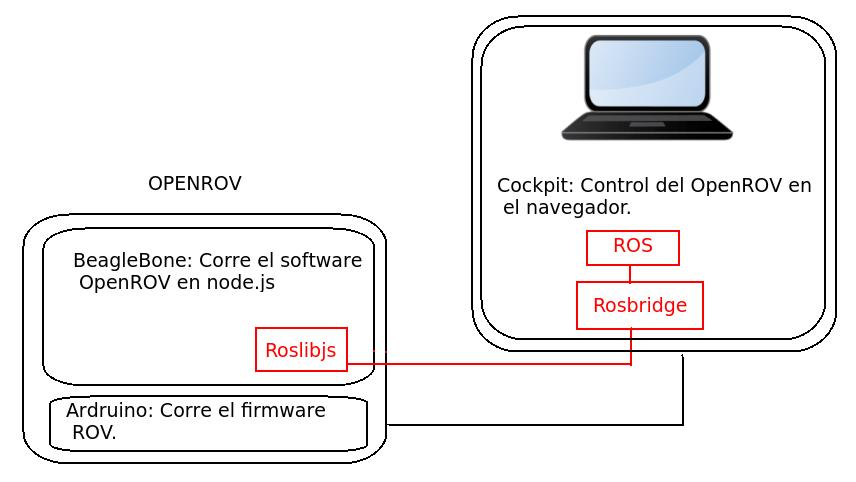
\includegraphics[width=8cm]{img/cap4/conect_ros_rov}
  \end{center}
  \caption{Diagrama de la conexión ROS y OpenROV}
  \label{fig:conect_ros_rov}
\end{figure}

La configuración del ROV implica la instalación de las dependencias para el complemento OpenROV. La principal dependencia para el plugin de ROV es roslibjs, sin embargo roslibjs también tiene varias dependencias.

Para empezar configuraremos la BeagleBone a través de una conexión SSH. Para ello necesitamos configurar el hardware del ROV de la siguiente manera:

\begin{enumerate}
\item Con un cable Ethernet, conectaremos el BeagleBone al router.
\item Utilizarmeos un cable mini USB para conectar el BeagleBone al portátil, de esta forma, activaremos el hardware.
\item Haremos un ssh hacia la BeagleBone, 
\renewcommand{\lstlistingname}{}
\begin{lstlisting}[caption=SSH, label={lst:ssh}]
$ ssh rov@192.168.7.2
\end{lstlisting}
cuando pida la contraseña, deberemos introducir “OpenROV”.
\end{enumerate}

\begin{figure} [hbtp]
  \begin{center}
    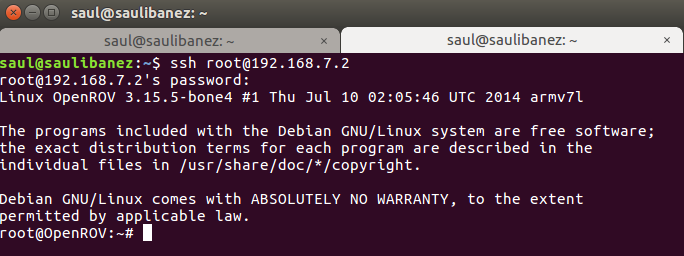
\includegraphics[width=12cm]{img/cap4/ssh}
  \end{center}
  \caption{SSH}
  \label{fig:ssh}
\end{figure}

Instalaremos las dependencias de Roslibjs, para ello ejecutaremos los siguientes comandos:

\renewcommand{\lstlistingname}{}
\begin{lstlisting}[caption=Dependencias Roslibjs, label={lst:roslibjs}]
sudo apt-get update 
sudo apt-get install libcairo2-dev libjpeg-dev libpango1.0-dev libgif-dev build-essential g++
\end{lstlisting}

\begin{figure} [hbtp]
  \begin{center}
    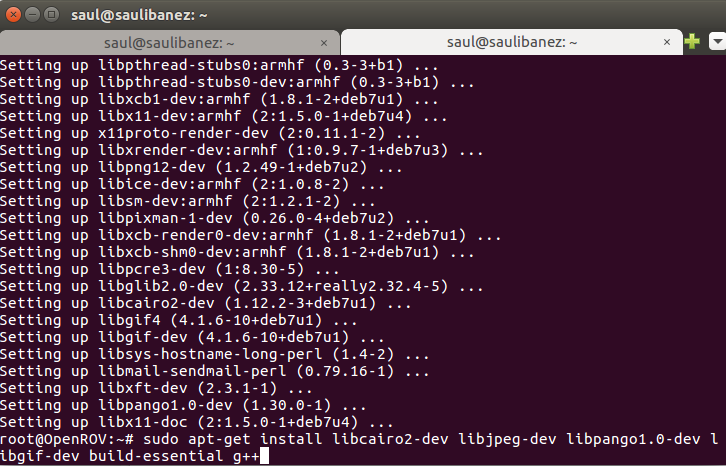
\includegraphics[width=12cm]{img/cap4/dependencias_roslibjs}
  \end{center}
  \caption{Dependencias Roslibjs}
  \label{fig:Dependencias Roslibjs}
\end{figure}

Seguidamente instalaremos otras dependencias (npm) de Roslibjs.
Para que no surjan problemas(errores del proxy), deberemos deshabilitar el proxy y realizar un reseteo del sistema. 
\renewcommand{\lstlistingname}{}
\begin{lstlisting}[caption=Dependencias Roslibjs, label={lst:roslibjs}]
sudo /etc/init.d/openrov-proxy stop
sudo /etc/init.d/openrov restart
sudo chown -R $USER /usr/local 
npm install canvas 
\end{lstlisting}

\newpage
\begin{figure} [hbtp]
  \begin{center}
    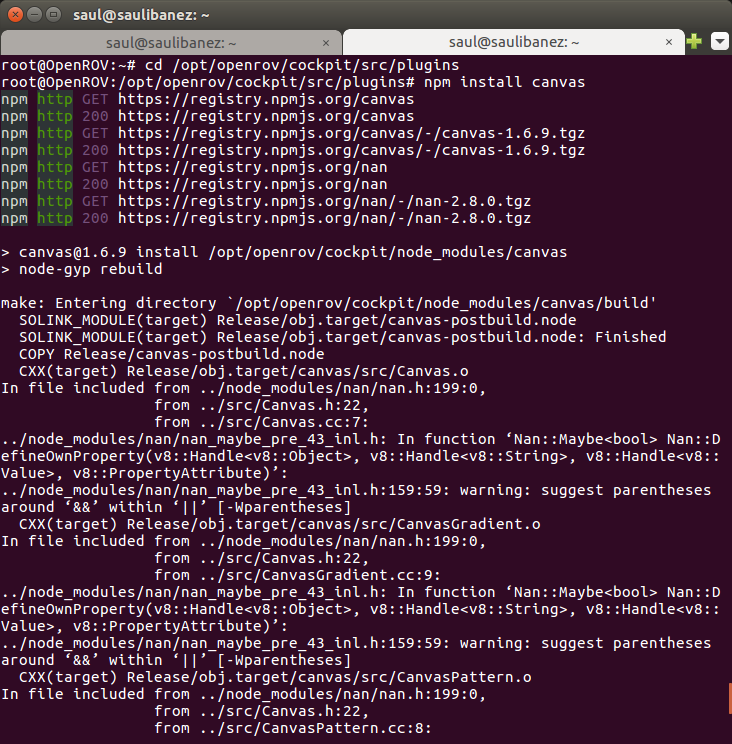
\includegraphics[width=12cm]{img/cap4/canvas}
  \end{center}
  \caption{Canvas}
  \label{fig:canvas}
\end{figure}

La última dependencia para el complemento es roslibjs, lo instalaremos usando: npm install roslib

Dentro de la carpeta /opt/openrov/cockpit/src/plugins se creará una carpeta llamada ros (sudo mkdir  ros) y en ella, crearemos un fichero index.js en el cual se ejecutará la conexión con el ROS Master.

\renewcommand{\lstlistingname}{}
\begin{lstlisting}[caption=Conexión con ROS, label={lst:conection_ros}]
function ros(name, deps) {
  		console.log("ROS plugin started");

  		// Comienza la sesion de ROS
 		var ROSLIB = require("roslib")
  		var ros = new ROSLIB.Ros({
    			url : 'ws://192.168.7.1:9090'
  		});

  		ros.on('connection', function() {
   			console.log('ROS connected to websocket');
  		});

  		ros.on('error', function(error) {
    			console.log('ROS error connecting to websocket');
  		});

 		 ros.on('close', function() {
    			console.log('ROS closed websocket connection');
 		});
	};

	module.exports = ros;
\end{lstlisting}

También se debe modificar el fichero hosts (sudo vim /etc/hosts) y en el realizaremos los siguientes cambios:

\begin{lstlisting}[caption=/etc/hosts, label={lst:hosts}]
#127.0.1.1	OpenROV
192.168.7.2	OpenROV
192.168.7.1	saul.ibanez.local
\end{lstlisting}

\section{Configuración de ROS}
\label{cap:Configuracion de ROS}
Antes de empezar cualquier conexión con ROS, deberemos instalarlo, en este punto, se ha decido instalar la distribucion de ROS Kinetic.

\begin{lstlisting}[caption=Instalacion de ROS, label={lst:install_ros}]
sudo sh -c 'echo "deb http://packages.ros.org/ros/ubuntu $(lsb_release -sc) main" > /etc/apt/sources.list.d/ros-latest.list'
sudo apt-key adv --keyserver hkp://ha.pool.sks-keyservers.net:80 --recv-key 421C365BD9FF1F717815A3895523BAEEB01FA116
sudo apt-get update
sudo apt-get install ros-kinetic-desktop-full
apt-cache search ros-kinetic
sudo rosdep init
rosdep update
echo "source /opt/ros/kinetic/setup.bash" >> ~/.bashrc
source ~/.bashrc
sudo apt-get install python-rosinstall python-rosinstall-generator python-wstool build-essential
\end{lstlisting}

Instalaremos Rosbridge
\begin{lstlisting}[caption=Rosbridge, label={lst:rosbridge}]
sudo apt-get install ros-kinetic-rosbridge-server
\end{lstlisting}

Cuando se configuró ROS, creamos una carpeta llamada catkin\_ws, en ella, se creó también la carpeta src, en la que crearemos el directorio openrov el que debe contener un fichero CmakeList.txt

El archivo CMakeLists.txt es la entrada al sistema de compilación CMake para crear paquetes de software. Cualquier paquete describe cómo crear el código y dónde instalarlo, el código será:

\begin{lstlisting}[caption=CMakeList.txt, label={lst:cmakelist}]
cmake_minimum_required(VERSION 2.8.3)
project(openrov)

find_package(catkin REQUIRED COMPONENTS
  	roscpp
  	rospy
  	std_msgs
 	sensor_msgs
  	geometry_msgs
  	message_generation
)

add_message_files(
    	FILES
    	navdata.msg
    	rovstatus.msg
   	motortarget.msg
  )

add_service_files(
    FILES
)

generate_messages(
	DEPENDENCIES
    	std_msgs
    	sensor_msgs
    	geometry_msgs
)

catkin_package(
   	INCLUDE_DIRS include
   	LIBRARIES openrov
   	CATKIN_DEPENDS roscpp rospy message_runtime
                  std_msgs sensor_msgs geometry_msgs
   	DEPENDS system_lib
)

include_directories(
  	${catkin_INCLUDE_DIRS}
)
\end{lstlisting}


Además, crearemos un directorio nombrado launch en el que se creará el fichero rosbridge.launch que contendrá:

\begin{lstlisting}[caption=websocket.launch, label={lst:launch}]
<launch>
 	<include file="$(find rosbridge_server)/launch/rosbridge_websocket.launch"/>
</launch>
\end{lstlisting}

Este código conduce a la instalación de rosbridge\_server e iniciará la conexión con ROV.

Para finalizar, y antes de ejecutar el .launch, deberemos ejecutar otro fichero, llamado set\_remote\_robot, el cual está configurado de la siguiente manera:
\begin{lstlisting}[caption=set\_remote\_robot, label={lst:remote}]
	export ROS_IP=192.168.7.1 	#YOUR IP
	export ROS_HOSTNAME=saulibanez.local 	#YOUR MACHINE
	export ROS_MASTER_URI=http://saulibanez.local:11311
\end{lstlisting}

\section{Conexión de ROS en OpenROV}
\label{cap:Conexion de ROS en OpenROV}

Habiendo realizado todos los pasos anteriores, ya estamos preparados para realizar la conexión de ROS en OpenROV.

Empezaremos conectando el OpenROV (solo con el cable MiniUSB en el portátil) abriremos un terminal y realizaremos un SSH a el BeagleBone (ssh rov@192.168.7.2).

Una vez conectados, desactivaremos el proxy (sudo /etc/init.d/openrov-proxy stop)y reinicamos elrobot (sudo /etc/init.d/openrov restart).

En otro terminal, ejecutaremos un roscore, que iniciará el ROS Master.

\begin{figure} [hbtp]
  \begin{center}
    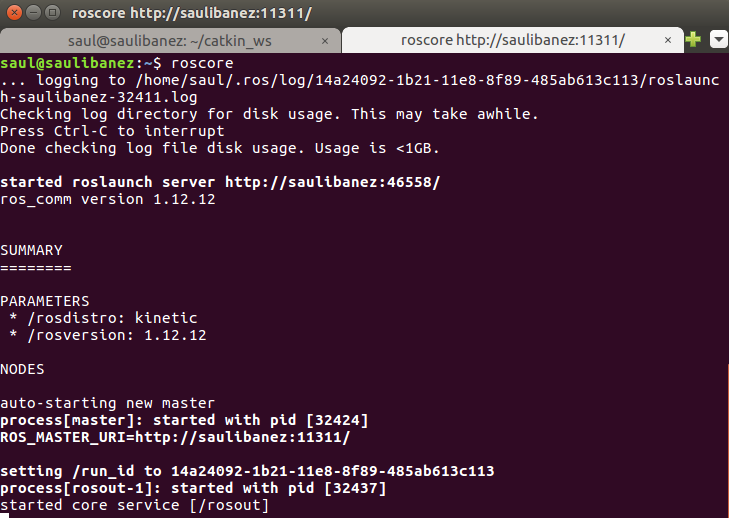
\includegraphics[width=11cm]{img/cap4/roscore}
  \end{center}
  \caption{Roscore}
  \label{fig:roscore}
\end{figure}
\newpage
Teniendo conectado el ROS Master, podremos ejecutar el launch rosbridge.launch, que es el que iniciará el nodo de rosbridge para comunicarse con OpenROV.

Ejecutando el código:
\begin{lstlisting}[caption=launch, label={lst:launch}]
	$ roslaunch openrov rosbridge.launch
\end{lstlisting}

\begin{figure} [hbtp]
  \begin{center}
    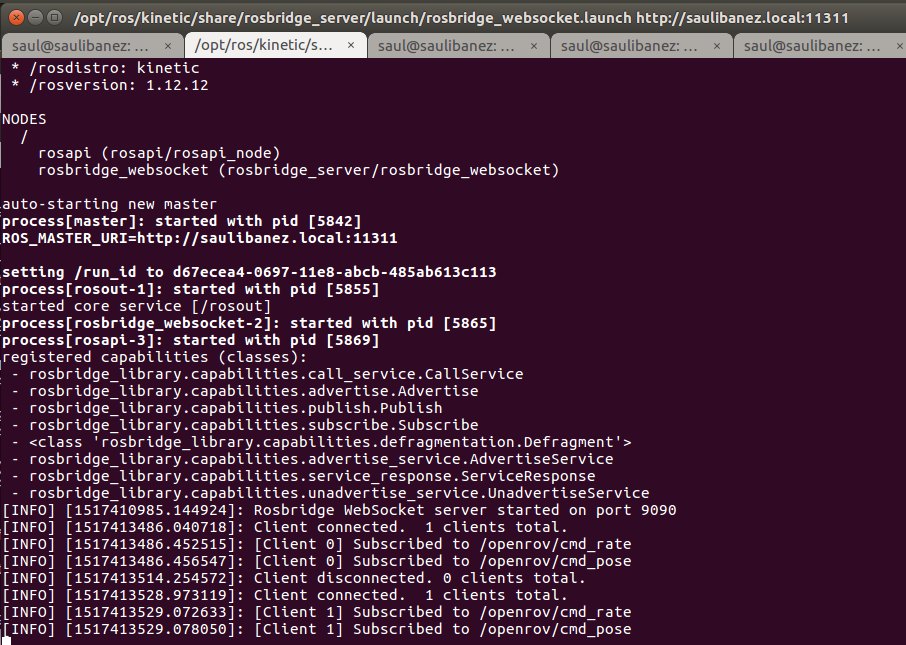
\includegraphics[width=11cm]{img/cap4/launch}
  \end{center}
  \caption{Launch}
  \label{fig:websocket.launch}
\end{figure}

También se comprobará en el terminal de OpenROV que la conexión se ha realizado

\begin{figure} [hbtp]
  \begin{center}
    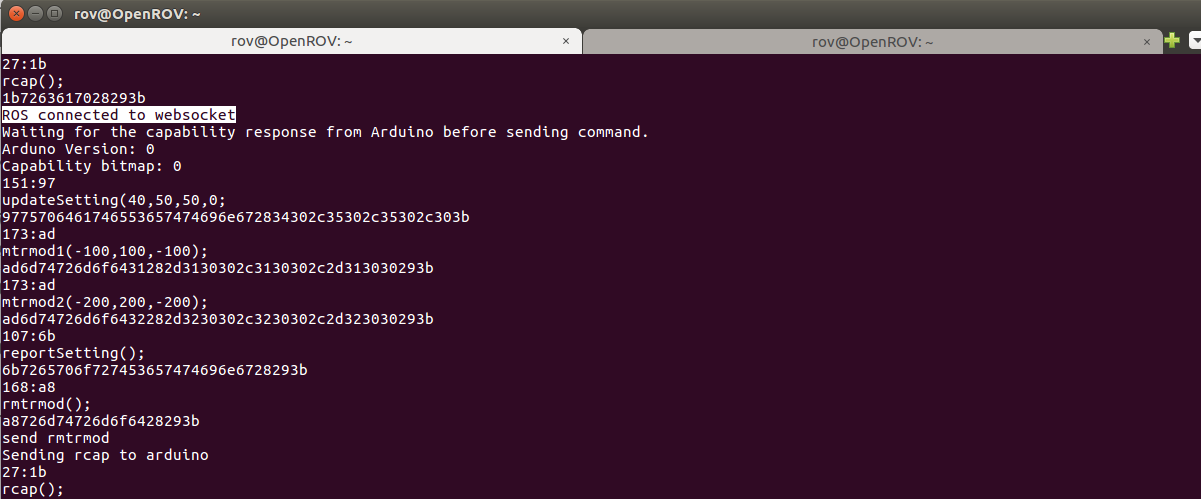
\includegraphics[width=12cm]{img/cap4/conexion_ROV}
  \end{center}
  \caption{Conexión en ROV}
  \label{fig:conect_rov}
\end{figure}

Para asegurarse de que todo esté funcionando, abrimos otra pestaña en el terminal e ingresaremos:
\begin{lstlisting}[caption=rostopic list, label={lst:list}]
	$ rostopic list
\end{lstlisting}

Esto mostrará una lista de los temas que están siendo publicados por el ROV, así como algunos temas predeterminados.

\begin{figure} [hbtp]
  \begin{center}
    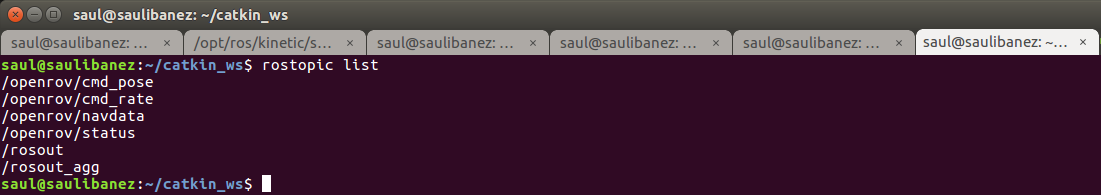
\includegraphics[width=12cm]{img/cap4/rostopic_list}
  \end{center}
  \caption{rostopic list}
  \label{fig:rostopic_list}
\end{figure}

Para ver información sobre el nodo en particular podremos ejecutar el comando :rostopic info.
\begin{lstlisting}[caption=rostopic info, label={lst:info}]
	$ rostopic info
\end{lstlisting}

\begin{figure} [hbtp]
  \begin{center}
    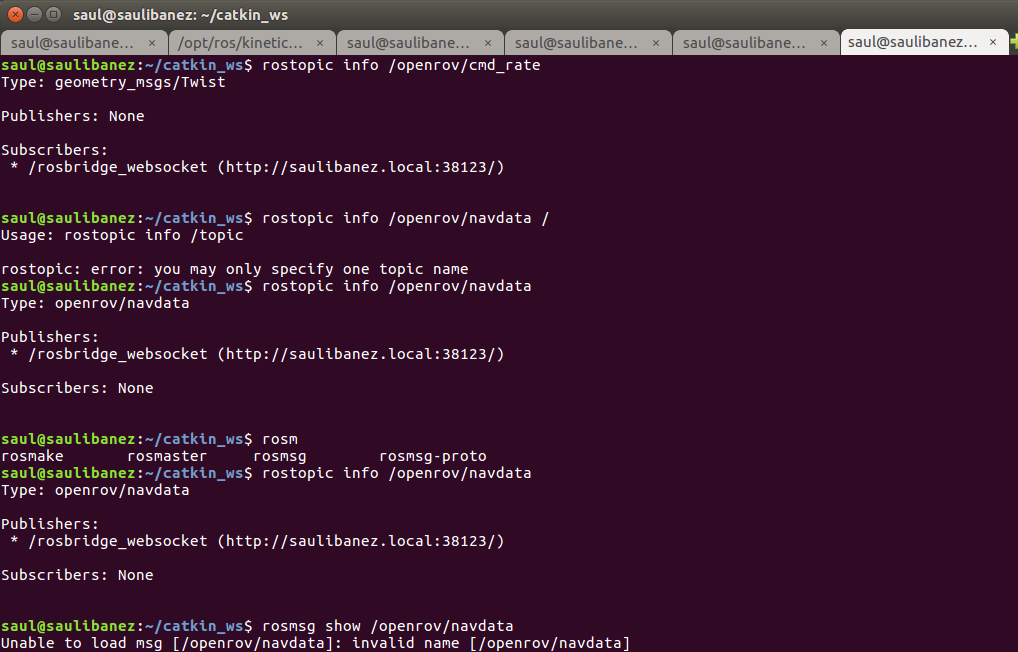
\includegraphics[width=12cm]{img/cap4/info1}
  \end{center}
  \caption{rostopic info (1)}
  \label{fig:rostopic_info}
\end{figure}
\begin{figure} [hbtp]
  \begin{center}
    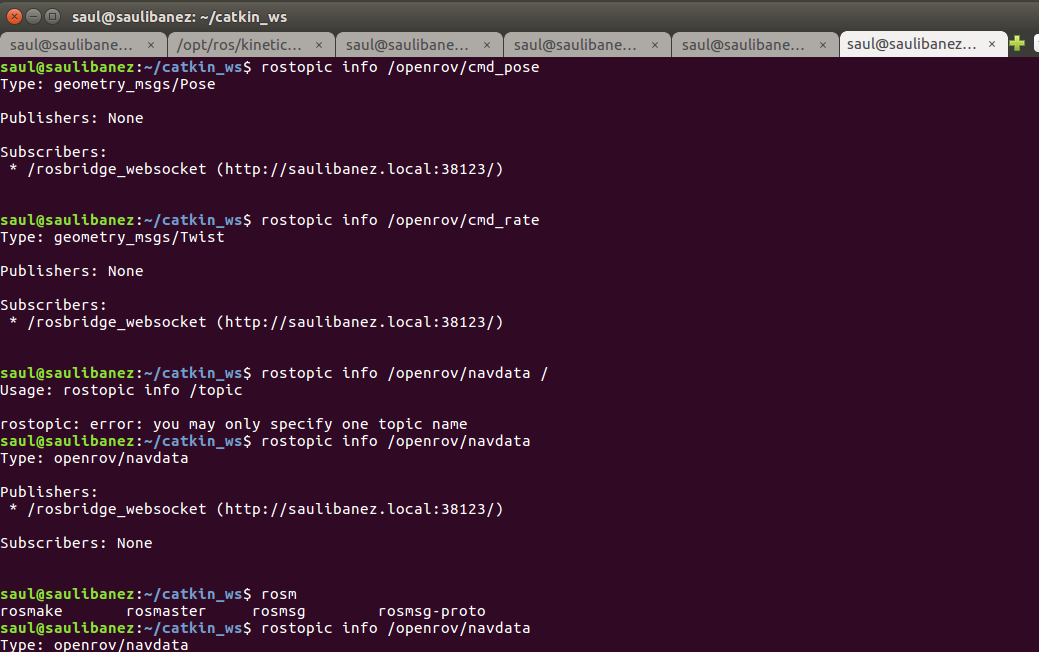
\includegraphics[width=12cm]{img/cap4/info2}
  \end{center}
  \caption{rostopic info (2)}
  \label{fig:rostopic_info}
\end{figure}